
\documentclass[a4paper,11pt]{article}
\usepackage[margin=1in]{geometry}


\usepackage[english]{babel}
\usepackage{amssymb}
\usepackage{amsmath}
\usepackage{amsfonts} 
\usepackage{graphicx}
\usepackage{sidecap}
\usepackage{mathtools}
%\usepackage{comment}
\usepackage{hyperref}
\usepackage{tikz}
\newcommand{\bulgr}{\textcolor{darkgreen}{$\bullet \;$}}
\newcommand{\bulor}{\textcolor{orange}{$\bullet \;$}}
\newcommand{\bulcy}{\textcolor{cyan}{$\bullet \;$}}
\newcommand{\bulbr}{\textcolor{brown}{$\bullet \;$}}
\newcommand{\ie}{{\itshape i.e. }}
\newcommand{\eg}{{\itshape e.g. }}

%opening
\title{\bfseries iTOP MCP-PMT module alignment method }
\author{A.Mord\'a}
\date{}
\begin{document}

\maketitle
\tableofcontents

\begin{abstract}
A procedure for the time alignment of the 512 MCP-PMT pixels installed in each of the 16 iTOP detector of Belle2 is presented. After a brief summary of the motivation and the alignment strategy, a data-driven procedure aiming to test the stability of the alignment method will be presented, along with the studies of simulated data that need to be used in the alignment procedure of the iTOP detector.
\end{abstract}

\section{Introduction}
The imaging Time Of Propagation (iTOP henceforth) detector provides Particle IDentification (PID) in the barrel region of the Belle2 detector. 
It is made of 16 modules, each of them consisting of:
\begin{itemize}
\item a 1.5 m long quartz bar
\item an expansion prism
\item an end plate array on the wider side of the expansion prism containing an array of 32 MCP-PMT produced by Hamamatsu
\item the readout electronic
\end{itemize}


The functioning principle is based on the folding of the Cherenkov cone generated by the charged particles ($\pi$, $K^\pm$) passing through the quartz bar.
The Cherenkov cone is reconstructed looking at the space-time pattern of the Cherenkov photons collected at the end-plate of the module. In particular, by knowing the charged track direction and the intersection point with the quartz bar is possible to analytically predict the space-time pattern of produced photon under different particle hypothesis, thus allowing to build a likelihood function that that can be used for the PID.

\begin{figure}
\begin{center}
\begin{minipage}{1\textwidth}
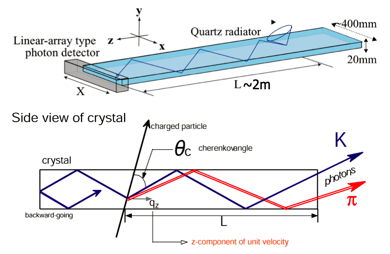
\includegraphics[width=0.7\textwidth]{pictures/BelleIIBPID3.jpg}
\caption{The working principle of the iTOP detector}
\label{fig:iTOP}
\end{minipage}
\end{center}
\end{figure}

\begin{figure}[t]
\centering
\begin{minipage}{0.4\textwidth}
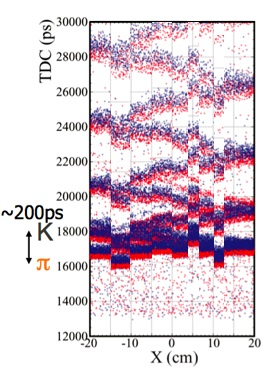
\includegraphics[width=\textwidth]{pictures/iTOP_pattern_noT0}
\caption{Time-space pattern of detected photon under different particle hypothesis, before the MCP-PMT pixels time alignment. For illustration only.}
\label{fig:PID_noT0}
\end{minipage}
\begin{minipage}{0.1\textwidth}
\end{minipage}
\begin{minipage}{0.4\textwidth}
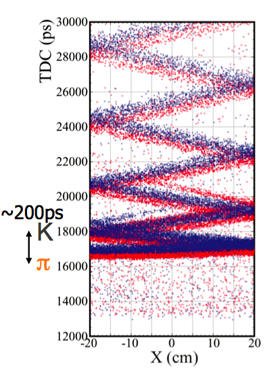
\includegraphics[width=\textwidth]{pictures/iTOP_pattern}
\caption{Time-space pattern of detected photon under different particle hypothesis, after the MCP-PMT pixels time alignment}
\label{fig:PID}
\end{minipage}
\end{figure}

\begin{subsection}{Motivations and strategy}
In order to produce a reliable PID an estimate as much as precisely as possible of the time offset ($T^0$ henceforth) of each MCP-PMT pixel is required. This offset originates from the different acquisition chains and properties of each pixels (such as the photo-electrons collection time). In the experiment this task is achieved by a Laser calibration system, already presented in \cite{Lasr_calib_syst_PD}. In the following the general strategy for the measurement of the $T^0$ will be presented in three steps: firstly showing the procedure in the ideal case, then in a {\itshape quasi}-real case, when including the effect due to quartz prism in between the light source and the PMT, and finally in the real case where many light sources illuminate the MCP-PMT array of the iTOP detector.

\paragraph{The time alignment (in principle)} In principle, the time alignment of the 512 pixels of each iTOP module can be done by illuminating all the MCP-PMT pixels with a synchronous light source (\eg a laser), and extracting the average detection time. In a given pixel, this is the sum of two contribution: the time offset $T^0_i$ and the light propagation time from the light source to the $i^{th}$ pixel:

\begin{equation}\label{eq:T0_def}
t_{(A,B)}=T^0_{(A,B)}+c_n^{-1} \cdot \ell_{(A,B)}
\end{equation}

or, equivalently

\begin{equation}\label{eq:delta_T0_def}
t_B-t_A=(T^0_B-T^0_A)+c_n^{-1}\cdot(\ell_B -\ell_A)\; ,
\end{equation}
being 
\begin{itemize}
\item $A$,$B$ two generic pixels,
\item $c_n$ the speed of light in the propagation medium,
\item $\ell_{(A,B)}$ the distance between the light source and the pixel $A$ and $B$,
\item $T^0_{(A,B)}$ the time off-sets of the pixels $A$ and $B$. 
\end{itemize}

A schematic scheme of this simple-case procedure is shown in fig.\ref{fig:cal1}.

 
\begin{figure}
\centering
\begin{minipage}{1\textwidth}
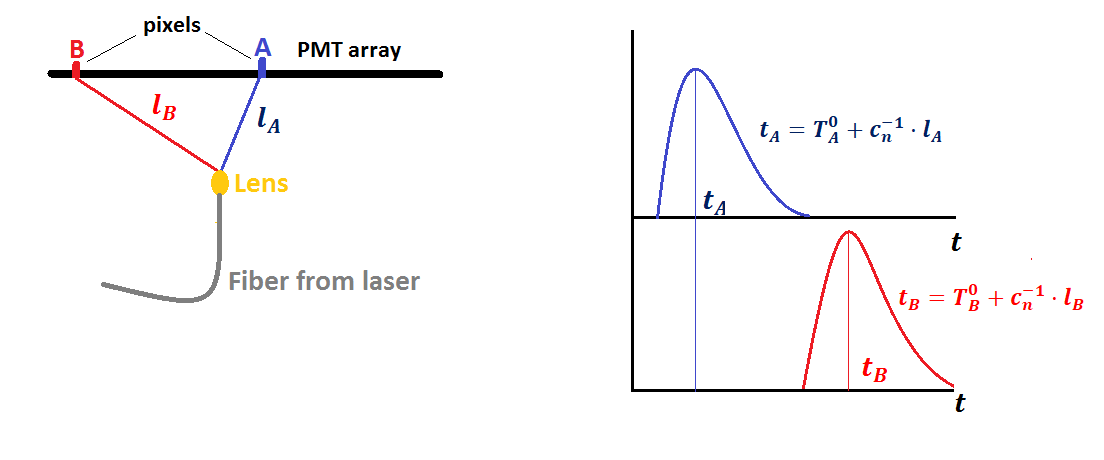
\includegraphics[width=\textwidth]{pictures/calibration_i}
\caption{The time alignment procedure in the ideal case.}
\label{fig:cal1}
\end{minipage}
\end{figure}


\paragraph{The time alignment (in {\itshape quasi}-practice)} In the experiment, the quartz expansion prism is placed between the light source and the MCP-PMT array. The effect of the quartz prism is that more a given pixel receives photons from different paths, because of refractions and reflections in the passage from air and the prism and inside the prism itself, as it is shown for illustration in fig.\ref{fig:cal2}.

\begin{figure}
\centering
\begin{minipage}{1\textwidth}
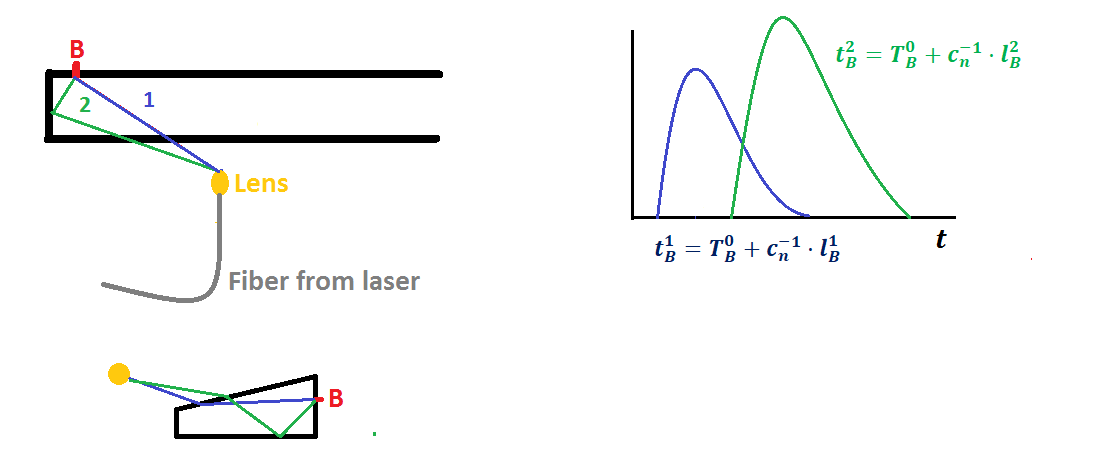
\includegraphics[width=\textwidth]{pictures/calibration_ii_0}
\caption{The time alignment procedure in the {\itshape quasi}-real case when the quart prism is inserted in between the light source and the MCP-PMT pixel.}
\label{fig:cal2}
\end{minipage}
\end{figure}


The fraction of each path depends on the properties of the lens (which is quite difficult to model with MC unless an excellent knowledge of lens properties is available); nonetheless, the position of the signal peaks is fixed only by the geometry of the propagation and is independent of the relative fraction of photon paths. The separation between two peaks is of the order of $\sim$ 200-300 ps, corresponding to path length differences within the prism of $\sim$ 5 cm. 


\paragraph{The time alignment (in practice)} The actual setup for the laser calibration consists of 9 light sources illuminating all the MCP-PMT of a module. For that reason, each MCP-PMT pixel receives light from more than one fiber, so that the actually observed time spectrum looks like the superposition of at least two of the profiles shown in previous paragraph, as illustrated in fig.\ref{fig:cal3}.


\begin{figure}
\centering
\begin{minipage}{1\textwidth}
\includegraphics[width=\textwidth]{pictures/calibration_iii}
\caption{The time alignment procedure in the real case where several fibers illuminate the MCP-PMT array through the quart prism.}
\label{fig:cal3}
\end{minipage}
\end{figure}




\end{subsection}

\begin{subsection}{The calibration setup}

\paragraph{KEK} The calibration system installed in the experiment consists of a Laser device acting as the synchronous source of photons. A mono-mode fiber, transmitting the laser photons up to the proximity of the iTOP module is then splitted into 16 fibers, one per each iTOP module, which carry the photon in the immediate vicinity of the modules; in turn, each of these 16 fiber is splitted into 9 multi-mode fibers, which are connected with a GRIN lens and which assures a uniform illumination of all the 32 MCP-PMT of each iTOP module. The choice of a mono-mode fibers for the first part of the transmittance is dictated by the necessity of reducing the light dispersion due to the propagation within the fiber. A scheme of the calibration system is shown in fig.\ref{fig:calKEK}.

In the calibration system of the experiment, all the fibers have been installed and fixed, and cannot be removed at our wish. For that reason it is not possible to study with true data which are the contributions to the detection time spectra due to a single fiber. Any information about the time detection spectra components must be then extracted from simulated data. 







\paragraph{Test-bench system} In order to carry more detailed studies on the time detection spectra model, and validate and test the procedure to extract the time offset of each pixel, a test-bench system, partially reproducing the one installed in the experiment, has been set up. Such a system allows, for instance, to inspect the contribution to the total time detection spectra originating from each single fiber, by acquiring data after the masking of one or more fibers.

The test-bench system consists of
\begin{itemize}
\item 1 MCP-PMT Hamamatsu
\item 1 SiPM fbk
\item a High Voltage supply device (providing to the MCP-PMT a voltage of 2500 V)
\item an amplifier (produced in Padova)
\item a digitizer CAEN V1742  at 5 GHz (16 + 1 trigger channels)
\item a PiLas laser device
\item the mono-mode fiber 
\item the multi-mode bundle
\item GRIN lens equals to those installed in the experiment
\item a prism equal to those installed in the experiment, rejected because of a production damage in one corner
\end{itemize}

The laser device provides also a trigger signal (as a step function) which is recorded as a waveform in a dedicated digitizer channel. All the computed detection times presented in the following sections are referred to the trigger time.

The signal detected by the photon detectors is digitized by the CAEN device, which provides, for each recorded event, a set of 1024 ADC values representing the signal waveform that will be processed for further studies. The time interval of one digitizer bin is 200 ps. The time window of one recorded signal is $\sim 200$ ns. 



\end{subsection}
\begin{subsection}{The calibration work flow}
In the following the main steps of the time alignment procedure will be presented.

\paragraph{Laser source characterization} A reliable time alignment requires first of all a comprehensive characterization of the light source. The main parameters that control the light emission from the Laser are the photon bunches emission frequency, the photon wavelength, and the attenuation factor (henceforth referred also as {\itshape tune}) which allows to modify the light yield. This attenuation coefficient is expressed as a percentage, and it has been verified that the relation between tune and light yield (defined as the number of photon observed per unit of time) is not linear, as it is shown in fig.\ref{fig:lightyield_vs_tune}. Many of the properties of the detection time spectra have been verified being strongly dependent on the tune value. For instance, the attenuation mechanism affects the laser time resolution, the average emission time of the light pulse, and causes the emission of photon with fixed delays with respect to the main bunches (seen as secondary peaks in the detection time distribution). A study of the photon detection time spectrum as a function of the tune has been done in order to fix the proper working point of the laser device. The results of such studies will be presented in sec.\ref{sec:laser_tune_study} 

\paragraph{Time spectra analysis} Once the light source has been characterized and the proper working point has been fixed, it is possible to run data acquisition, as previously explained, reconstruct the photons detection time spectra, and proceed with the data analysis, whose goal is the definition of the pixel time offset measurement procedure. This consists in defining a model to describe the observed spectra and use it to fit for the position of a given photon path (henceforth referred to as the {\itshape calibration peak} or {\itshape signal}). In principle, the separation between the arrival time of different photon paths can be fixed analytically or looking at simulated data; this is suitable in order to reduce the number of free parameters in the fit to the observed spectra, leaving the resolutions of the observed photon paths, their relative weight, the calibration peak position, and few more nuisance parameters (such as noise and signal shapes related quantities) as free parameters of the model. Once the position of the calibration peak has been measured, the position of the corresponding peak in simulation must be subtracted to get the time offset of the considered pixel. 

In the real case, nevertheless, the simulated data are not guaranteed to fully reproduce the time distribution of all the optical paths that actually reach a given MCP-PMT pixel (basically because of an approximate knowledge of the lens orientation and properties, such as the opening angle). For instance, they can predict a non-negligible contribution of a given photon path which turns out to be negligible in the true data; or, {\itshape vice-versa}, the simulation can predict that a given photon path contribution is negligible while this is not the case in the true data. In addition, even assuming that the simulation properly reproduces the observed pattern, the geometry of the system makes the distance between the different path arrival times getting too small for some pixels, so that it is only possible to align the measured position of the {\itshape calibration peak} in the observed spectra with an average of the positions observed in the simulation, thus affecting the ultimate resolution on the {\itshape calibration signal} position. 

From what has been said before, a detailed study of the simulated data is required, in order to figure out which quantities can be used as input for the fit, and which is the ultimate uncertainty on the time offset arising from a possible mismatch between the calibration peak defined in data and the corresponding one identified in simulation.

In the following, two different (thought complementary) approaches through which defining the time offset measurement will be presented.

\paragraph{Data-driven procedure} With this approach, the model for the observed spectrum in a given pixel is built looking at the contributions originating from each single fiber. For that reason this method can be applied only on the test-bench system and is meant to check the stability of the procedure to extract the position of a given photon path, position that will be compared to the corresponding one in the simulated data in order to extract the time offset. 

To check the stability of the procedure, the position of the calibration peak is measured in two conditions: through a fit to the spectrum $\mathcal{S}_c$ observed with the fiber the calibration signal originates from, and after adding to $\mathcal{S}_c$ the contribution of the adjacent fiber $\mathcal{S}_a$. The geometrical quantities, such as the separation between any pair of peaks, are fixed by fitting separately the spectra observed with each of the two fibers $\mathcal{S}_{(c,a)}$; the measured values are used as inputs for the fit of the full spectrum $\mathcal{S}_T$ obtained with both fibers. If the positions of the calibration peak in the two conditions are compatible with each other, then the procedure can be considered reliable; in addition this procedure helps understanding how stable the fit model is (provided reasonable inputs are provided, either from simulations or from real data) and possibly defining a suitable calibration peak, as the one undergoing the smaller variation when the noise due to optical paths from adjacent fibers is added. The clear advantage of this method is that it is completely data-driven, thus removing the uncertainties due to approximated knowledge of lens opening angle, which is needed to generate the simulated datasets: the separation between peaks is extracted directly from data and already includes the effects due to the relative photon path weights \footnote{As well as the differences arising from paths reaching the upper and lower edges of the pixel} on the separation between two peaks.

%In more details an {\itshape ansatz} is done, assuming that only two paths contribute to the observed spectra obtained with only one fiber.

\paragraph{MC based procedure} This is the actual procedure that will be used for the calibration of the iTOP. Indeed, in the experiment, it is not possible to remove the fibers, so that the only observable spectra are the superposition of the contributions originating from each of the fibers whose emitted photons reach the pixel. In this conditions the geometrical quantities that must be used as inputs of the fit by which measuring the position of the calibration signal (such as the time separation between two optical paths) must be extracted from simulation. Nevertheless, the mismodel of the lens opening angle can cause the simulated spectra differing from those really observed for some photon paths, as already explained. For that reason a detailed study of the simulated data, as well of the fit procedure, is required in order to understand what kind of inputs can be extracted from the MC and which is the maximal numbers of model parameters that can be left free in the fit to the time spectra.  All those quantities will affect the ultimate resolution on the calibration peak, and, in turn, the quality of the alignment constants and of the PID variables. 


\end{subsection}

\section{The laser device characterization}\label{sec:laser_tune_study} 

The light yield of the laser device can be tailored through an internal attenuation mechanism. This mechanism, depending on the required attenuation value, can drastically affect the properties of emitted bunches of photons, in particular the average photon emission time, the resolution of the emission time distribution, and the emission of photon with a delay, with respect to the main time, of the order of $\sim$ 4 ns.

To study the effects of laser tune values on the properties of the emitted photon bunches a data campaign has been done, by acquiring data at different values of the laser tune and using two configurations of the setup:
	\begin{itemize}
		\item SiPM (fbk) without the quartz bar; 
		\item MCP-PMT (High Voltage supply at 2500 V) and quartz bar in between fiber and MCP-PMT.
	\end{itemize}
In both cases, the signal from the photon detector has been read {\it as it is}, namely without being amplified, in order to reduce as much as possible the time spread introduced by additional electronic devices in the acquisition chain. 

The use of the two above mentioned setup is dictated by the fact that the SiPM can work fine also in a multi-photon regime; the MCP-PMT, instead, has been designed to work in a single-photon regime and features an unstable behavior when the light intensity is increased. This makes the SiPM more suited to acquire data at low laser tune values, thus allowing to scan over a wider range of laser tune values. The use of the MCP-PMT setup is instead dictated by the smaller recovery time of such detector with respect to the SiPM, which allows, as it will be discussed later, to examine the appearance of delayed light pulses from the laser.% Nonetheless, the time resolution of the SiPM at high laser tune vales is very large ($\sim 450$), and its large recovery time makes impossible to determine the position of the delayed pulses; to this extent the MCP-PMT is more suited, provided the light intensity is kept enough low to guarantee a single-photon regime.


In total 30 (16) datasets for each laser tune value have been acquired using the SiPM (MCP-PMT) photon detector.
The setup with the laser light directly illuminating the SiPM has been used to study the dependence of the $T^0$ and the laser time resolution on the laser tune value; the configuration with the MCP-PMT, together with the quartz expansion prism, is used to study the relation between the yield of delayed emitted photons and the tune value. 
	
\begin{subsection}{Absolute $T^0$ and laser resolution}
To study the dependence on the laser tune value of the mean emission time and the time resolution of the laser device, 30 datasets have been acquired at different tune values, from 96\% to 50\%, in steps of 2\% in the ranges 50\%-68\% and 84\%-96\%, and in steps of 1\% in the range 70\%-82\%.
The distribution of the maximal amplitude of the SiPM signal is reported in fig.\ref{fig:SiPM_tune_scan_amp}. From values of the tune $\simeq 76\%$ the maximal amplitude of the SiPM signal saturates, because of the loose of the single photon regime. The detection time is computed as follow:
\begin{itemize}
\item a scan over the signal waveform is done until a maximum has been found;
\item the average level of the noise is computed by averaging over the first samples of the recorded waveform;
\item the position of the detection time is computed as a weighted average (over the corresponding waveform values) of the two sample points above ad below 50\% of the maximum amplitude (noise subtracted). 
\end{itemize}

The distribution of the observed time spectra is shown in fig.\ref{fig:SiPM_tune_scan_T}. In order to measure the position of the detection time and the width of the distribution, the observed spectra have been fitted with a gaussian function. Due to the negligible level of noise, any component has been used to describe its contribution.  

The dependence of the measured $T^0$ and laser time resolution are summarized in plots in figg.\ref{fig:SiPM_Tdistr}-\ref{fig:SiPM_sigmadistr}. Both the emission time $T^0$ and the laser time resolution are observed varying significantly with the laser tune. Even thought the dependence of the $T^0$ is not really relevant to fix the working point of the laser, the strong dependence of the laser emission time resolution with the tune sets strong constraints on the tune value to be used. Optimal values are below $\sim 76\%$, since in that region the time resolution saturates at values (around $\sim 10$ ps) which are well below the full MCP-PMT time resolution target of $\sim 100$ ps. Remarkably, such a value for the time resolution is also well beyond the one provided by the constructor, who guaranteed a laser time resolution of $\sim 25$ ps for tune values of 50\%. 

\begin{figure}
\begin{center}
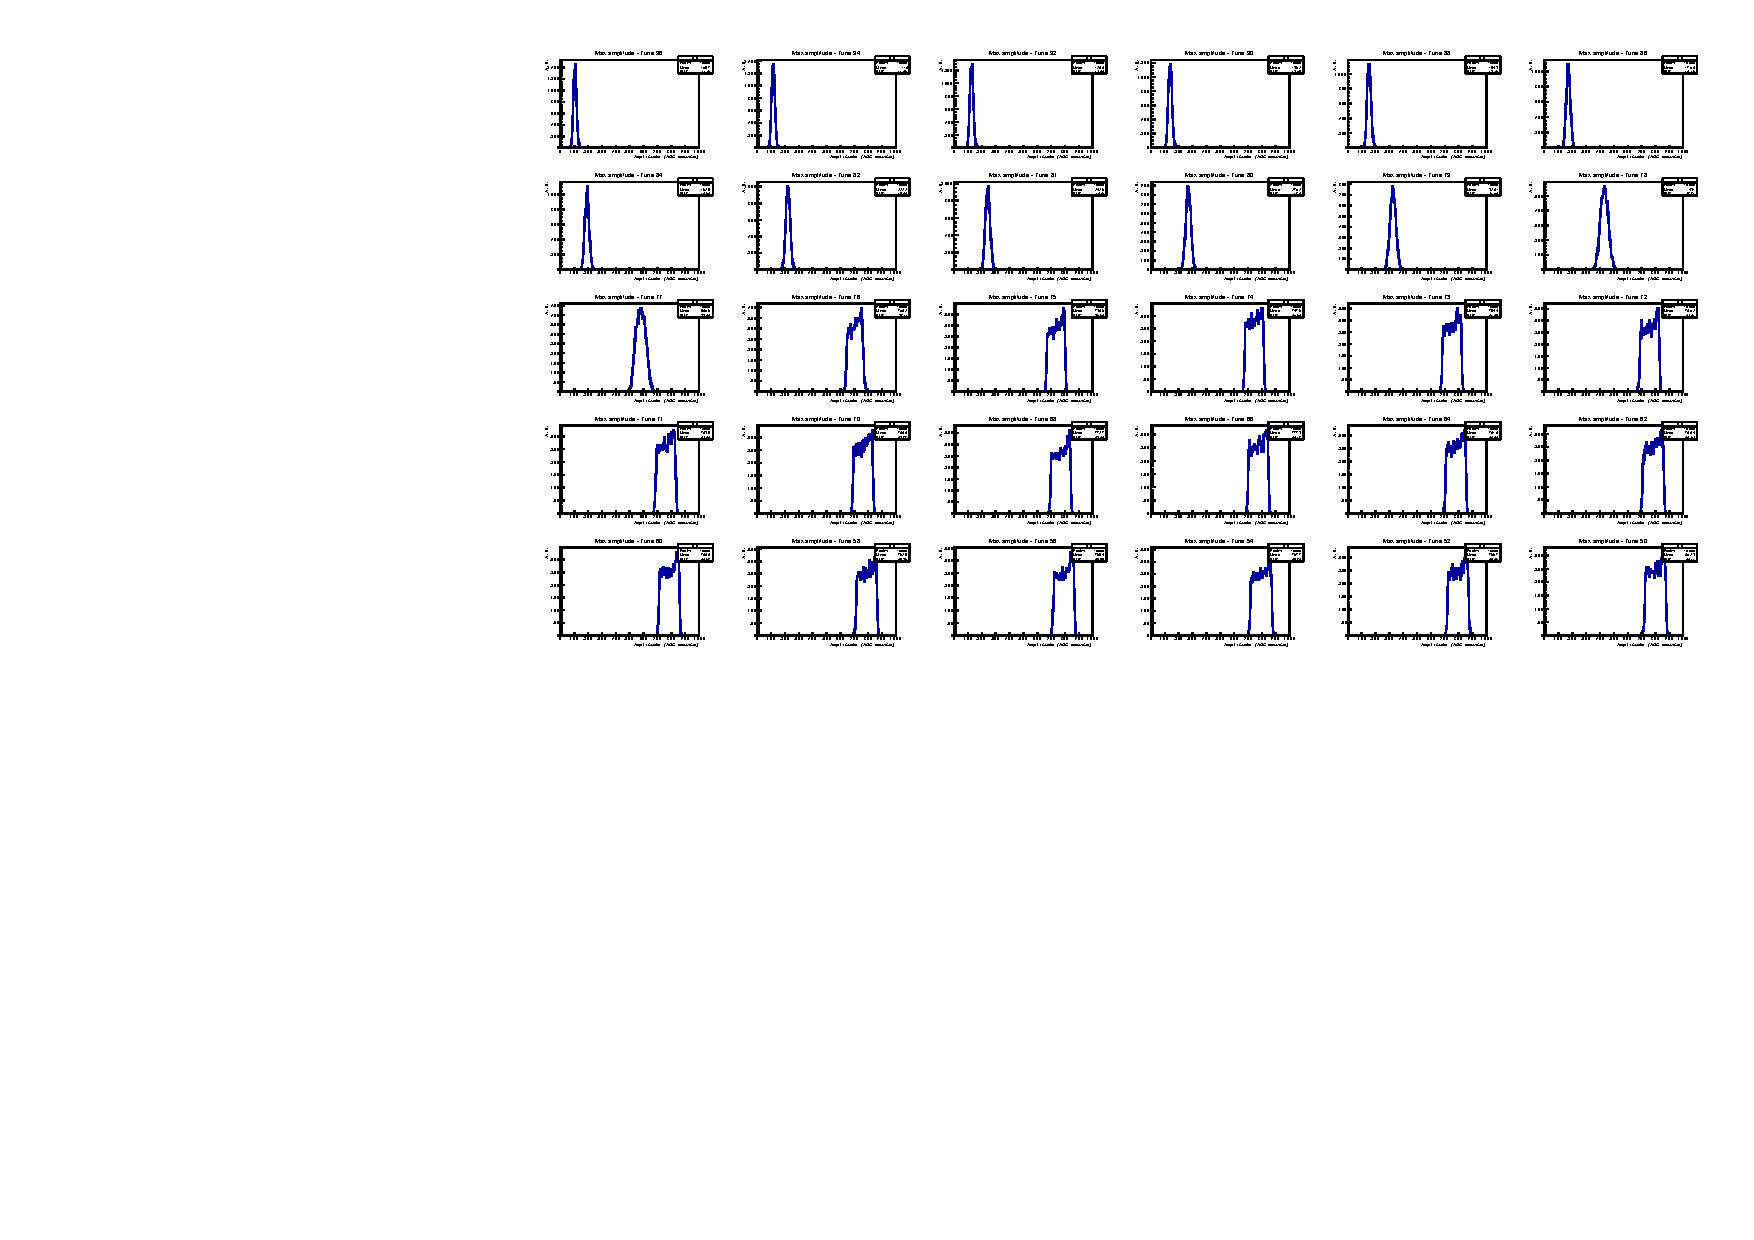
\includegraphics[scale=0.8]{plots/SiPM_ampdistr}
\caption{Distribution of the maximal amplitude (in ADC counts) of the signal waveform for the 30 datasets (each of them corresponding to a different value of the laser tune) acquired with the SiPM. From tune values of $\sim 76\%$ the amplitude saturates because of the loose of the single photon regime.}
\label{fig:SiPM_tune_scan_amp}
\end{center}
\end{figure}

\begin{figure}
\begin{center}
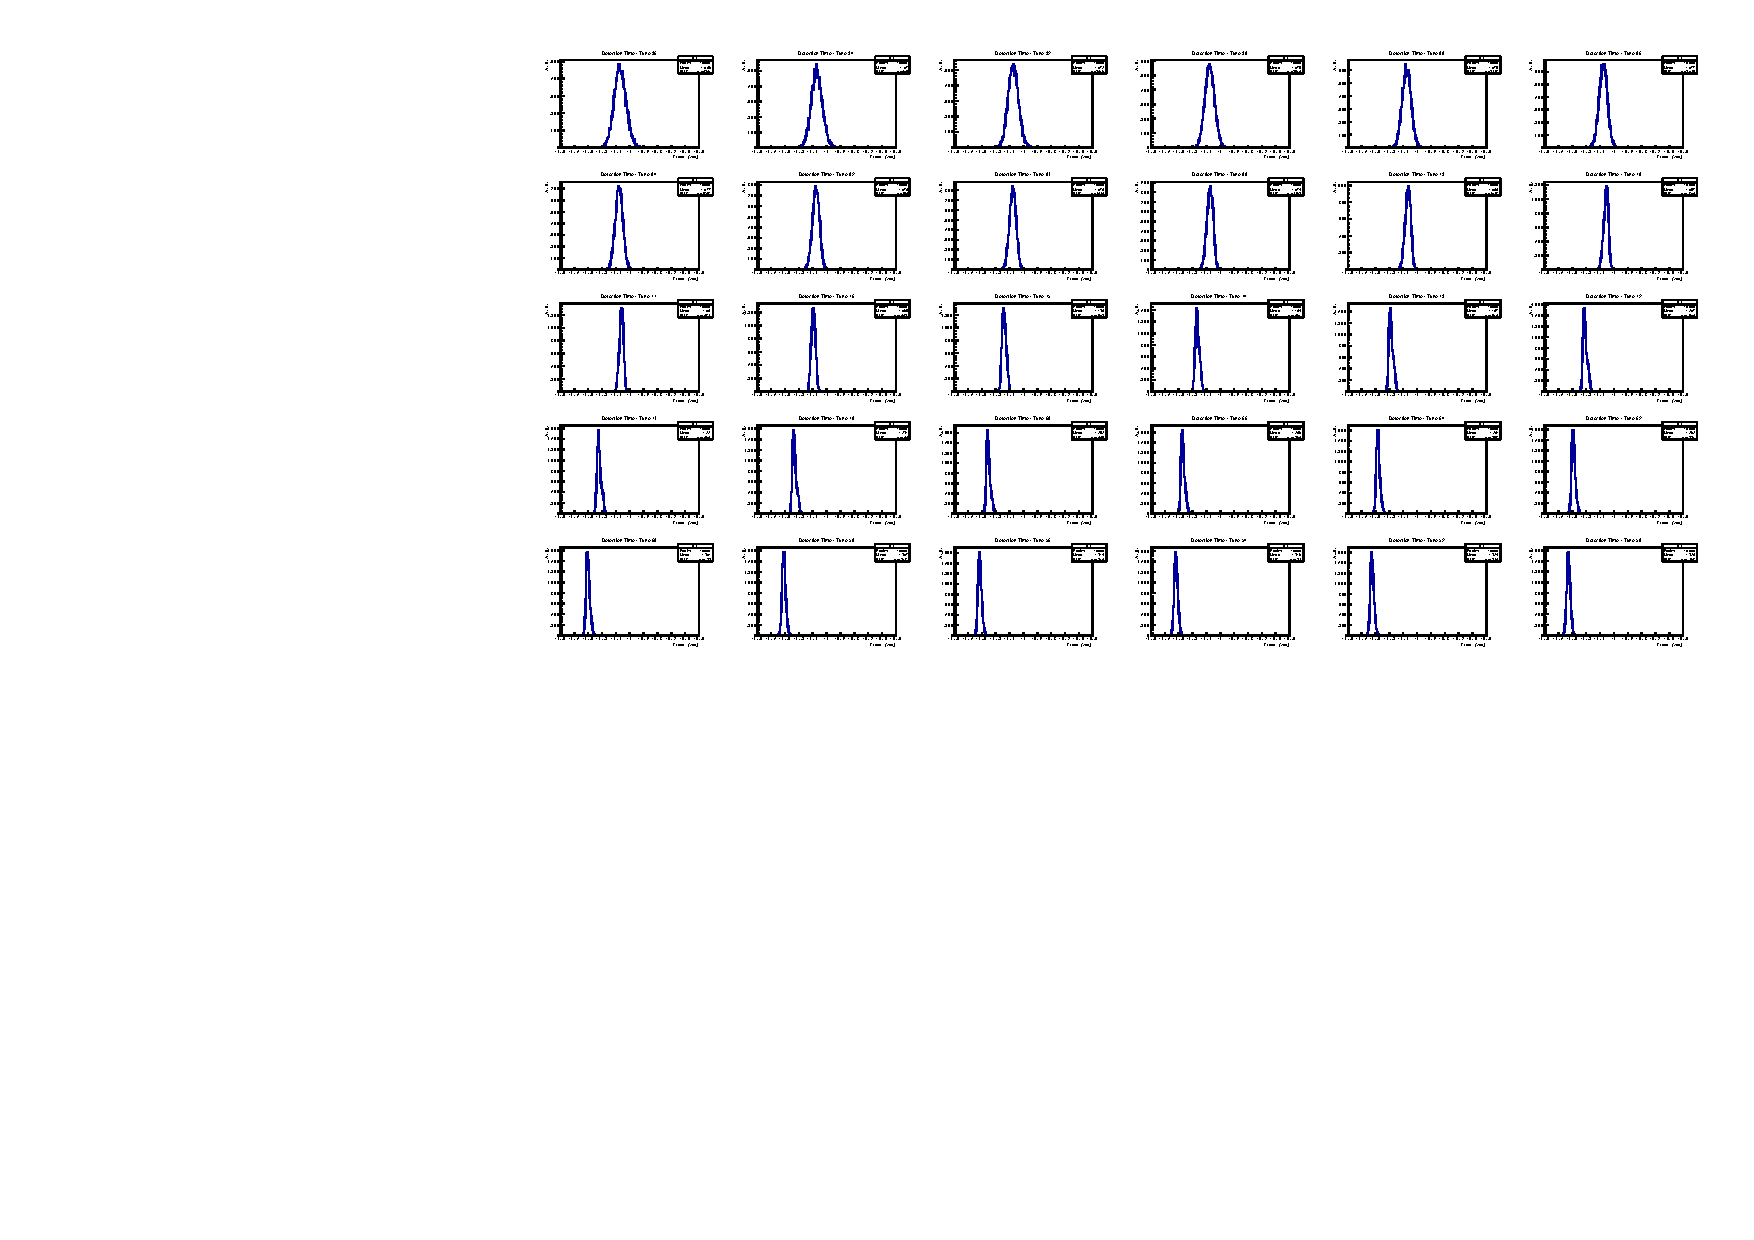
\includegraphics[scale=0.8]{plots/SiPM_Tdistr}
\caption{Distribution of the detection time (expressed in [ns] and computed with respect to the laser trigger signal) of the emitted photons observed in the 30 datasets (each of them corresponding to a different value of the laser tune) acquired with the SiPM. The x axis range is [-1.5,0.5] ns.}
\label{fig:SiPM_tune_scan_T}
\end{center}
\end{figure}


\begin{figure}
\begin{center}
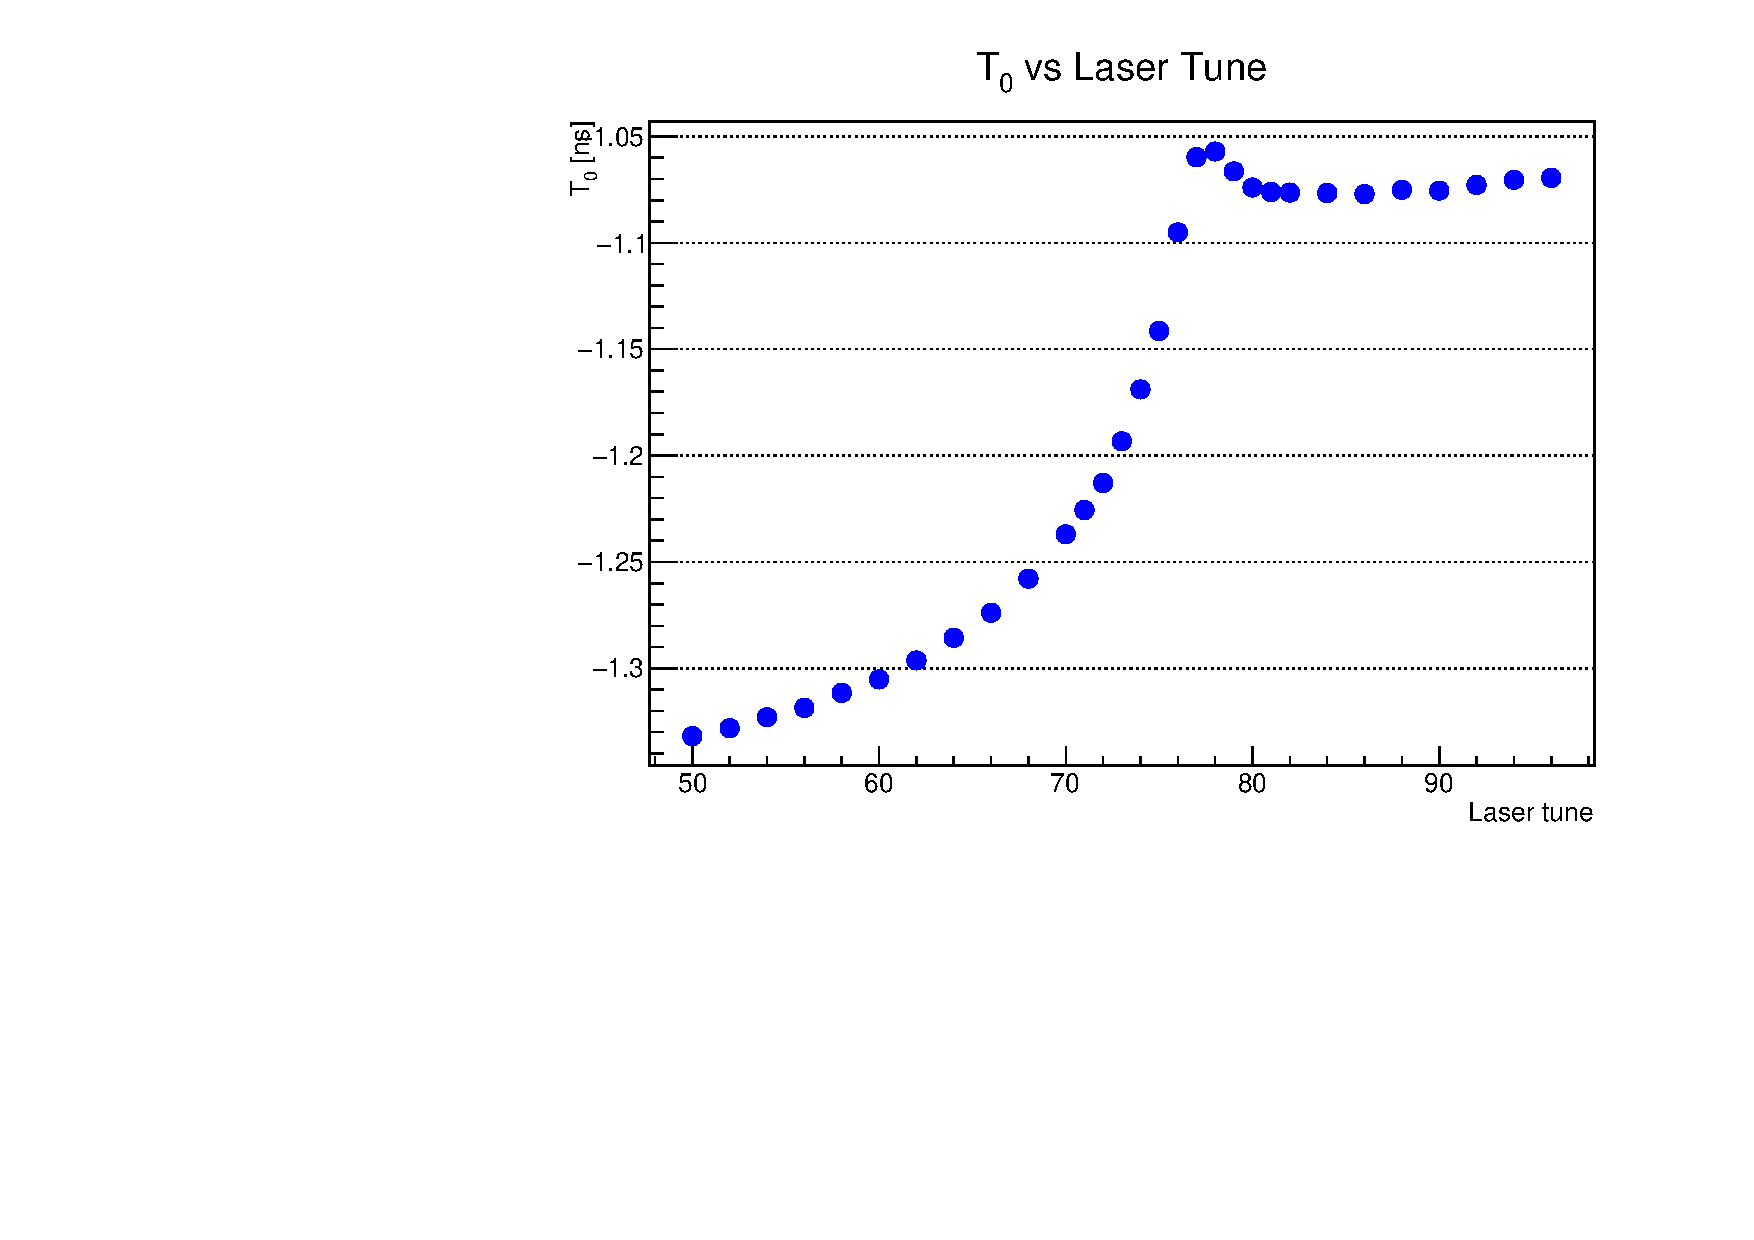
\includegraphics[scale=0.7]{plots/SiPM_T0distr}
\caption{Value of the mean emission time of the laser (measured through a fit to the detection time spectra observed with the SiPM) as a function of its tune (30 values). The error bars are within the point sizes.}
\label{fig:SiPM_Tdistr}
\end{center}
\end{figure}
\begin{figure}
\begin{center}
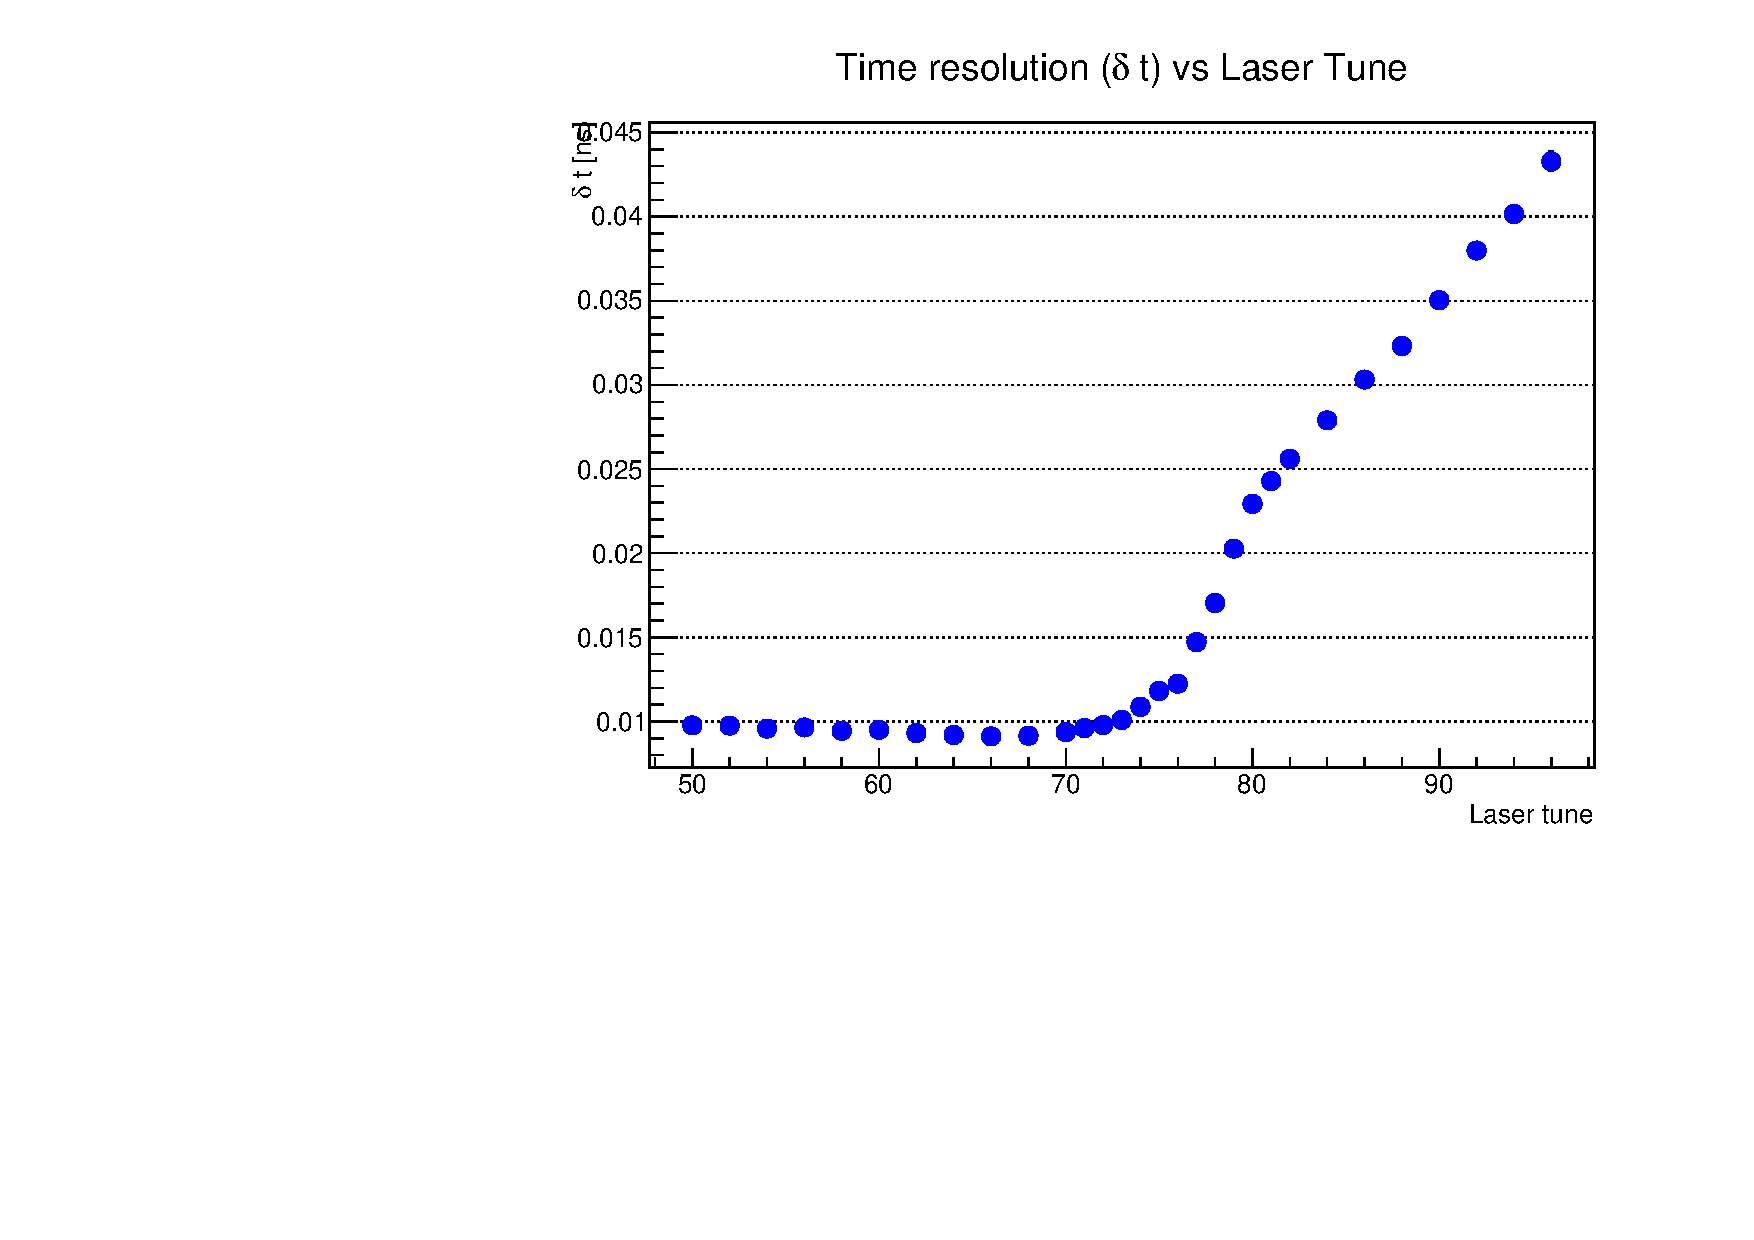
\includegraphics[scale=0.7]{plots/SiPM_res0distr}
\caption{Value of the time resolution of the laser emitted photons (measured through a fit to the detection time spectra observed with the SiPM) as a function of its tune (30 values). The error bars are within the point sizes.}
\label{fig:SiPM_sigmadistr}
\end{center}
\end{figure}

\paragraph{Discussion about detection time computation and delayed pulses}The choice of looking at the position of the first maximum of the signal waveform is dictated by the interest in the position of the first bunch of photons emitted by the laser. Moreover in the ideal case the signal waveform is expected to feature only one maximum, generated by the detection of the photon in the SiPM device. Nevertheless, in the reality, this is not always the case, since some delayed light pulses are observed either as secondary peaks in the recorded waveform or as shifted waveform. In the former case, the signal corresponding to the delayed photons appears as secondary peaks on top of the first detected light pulse tail, and in some cases their absolute amplitude can be larger than the one of the first maximum, as it is shown in figg.xx-yy. For that reason they appear in the absolute time spectrum as secondary peaks at fixed distances from the main signal. The determination of the detection time of these peaks with a Constant Fraction Method, as it was done for the first waveform maximum, is not straightforward (it would require a fit of the first signal tail, for instance). The study of such secondary pulses and their correlation with the laser tune value has been performed using the MCP-PMT, which has a much shorter recovery time with respect to the SiPM and allows to better separate the direct and delayed light pulses.
\end{subsection}


\begin{subsection}{Secondary peaks in detection time spectra}

The study of the delayed pulses as a function of the laser tune are based on a data campaign consisting of 16 datasets acquired with different values of he laser tune in the range 72\%-90\%; in more details, in the range 72\%-82\% a tune difference of 1\% has been used, while in the range 84\%-90\% the tune differences are of 2\%. 


For the MCP-PMT the signal waveform consists of one or more signal peaks, enough separated with each other to allow a reliable determination of the detection time of the different photon signals with a Constant Fraction method. For that reason, differently from what has been done with the data acquired with the SiPM, there could be more detection times in the same event, depending on the presence of delayed emitted photons.

The MCP-PMT receives the photons coming out of the expansion prism\footnote{The use of the quartz prism for this data campaign has been dictated by the necessity to avoid (or reduce as much as possible) any mechanical displacements of the test-bench system.}, so that the detection time spectra will feature several structures: 
\begin{itemize}
\item a large statistics peak in correspondence of the main laser emission time. This main peak is actually the superposition of two or more elementary peaks corresponding to the different photon paths within the prism. The time difference between two peaks corresponding to different photon paths is no larger than $\sim 350$ ps and depending on the laser tune value (which, according to what has been previously shown, affects the time resolution of the emitted photons) such substructures can be more or less evident;
\item more secondary peaks, evident for times larger than $\sim 4$ ns with respect to the central position of the main peak and which appear as a consequence of the delayed emission of photon. Even though these secondary peaks could feature some substructures due to the different photon paths inside the prism (as it happens for the main peak), these are never resolved, because of the small statistics of the peaks and a very large time resolution of such delayed photon bunches.
\end{itemize}





Three of the time spectra acquired in one of the 16 MCP-PMT pixels are reported in fig.\ref{fig:SP_MCPPMT_T86}-\ref{fig:SP_MCPPMT_T77} together with the results of the fit used to measure the properties of the spectra, among which there is the total fraction of main photon signals $F_{sig}$. The model used to fit the observed distributions consists of a signal component (a linear combination of two {\it Crystal Ball} \footnote{See next section}), a component describing the secondary peaks and a noise function (modeled by a second degree Chebychev polynomial). The latter gives always a negligible contribution to the total spectrum; the component modeling the delayed emission structures consists of three components (each of them being a Landau function, whose use is justified by the asymmetry of the shape of the two evident delayed peaks at times larger than 4 ns): the second and third of these components are reasonably due to the delayed emission while the first of these components is centered on the tail of the main signal peak, and could be interpreted as well as a third component of the main peak signal arising from a third photon path in the expansion prism. Nevertheless, being its contribution negligible with respect to the one of the two main signal peaks, it has been considered, in a conservative approach, as a delayed peak at a distance with respect to the signal peak smaller than 4 ns.

The dependence of $F_{sig}$ as a function of the attenuation value of the laser is reported for the 16 laser tune value acquisitions in fig.\ref{fig:SP_MCPPMT}. The total fraction of secondary peaks (defined as $1-F_{sig}$) undergoes a significant non linear variation with the laser tune. At high values of the attenuation it can account for up to $\sim$ 25\% of the total number of observed photon signals. As the tune gets smaller the fraction saturates at negligible values from attenuation values of $\sim$ 76\%.


\begin{figure}
\begin{center}
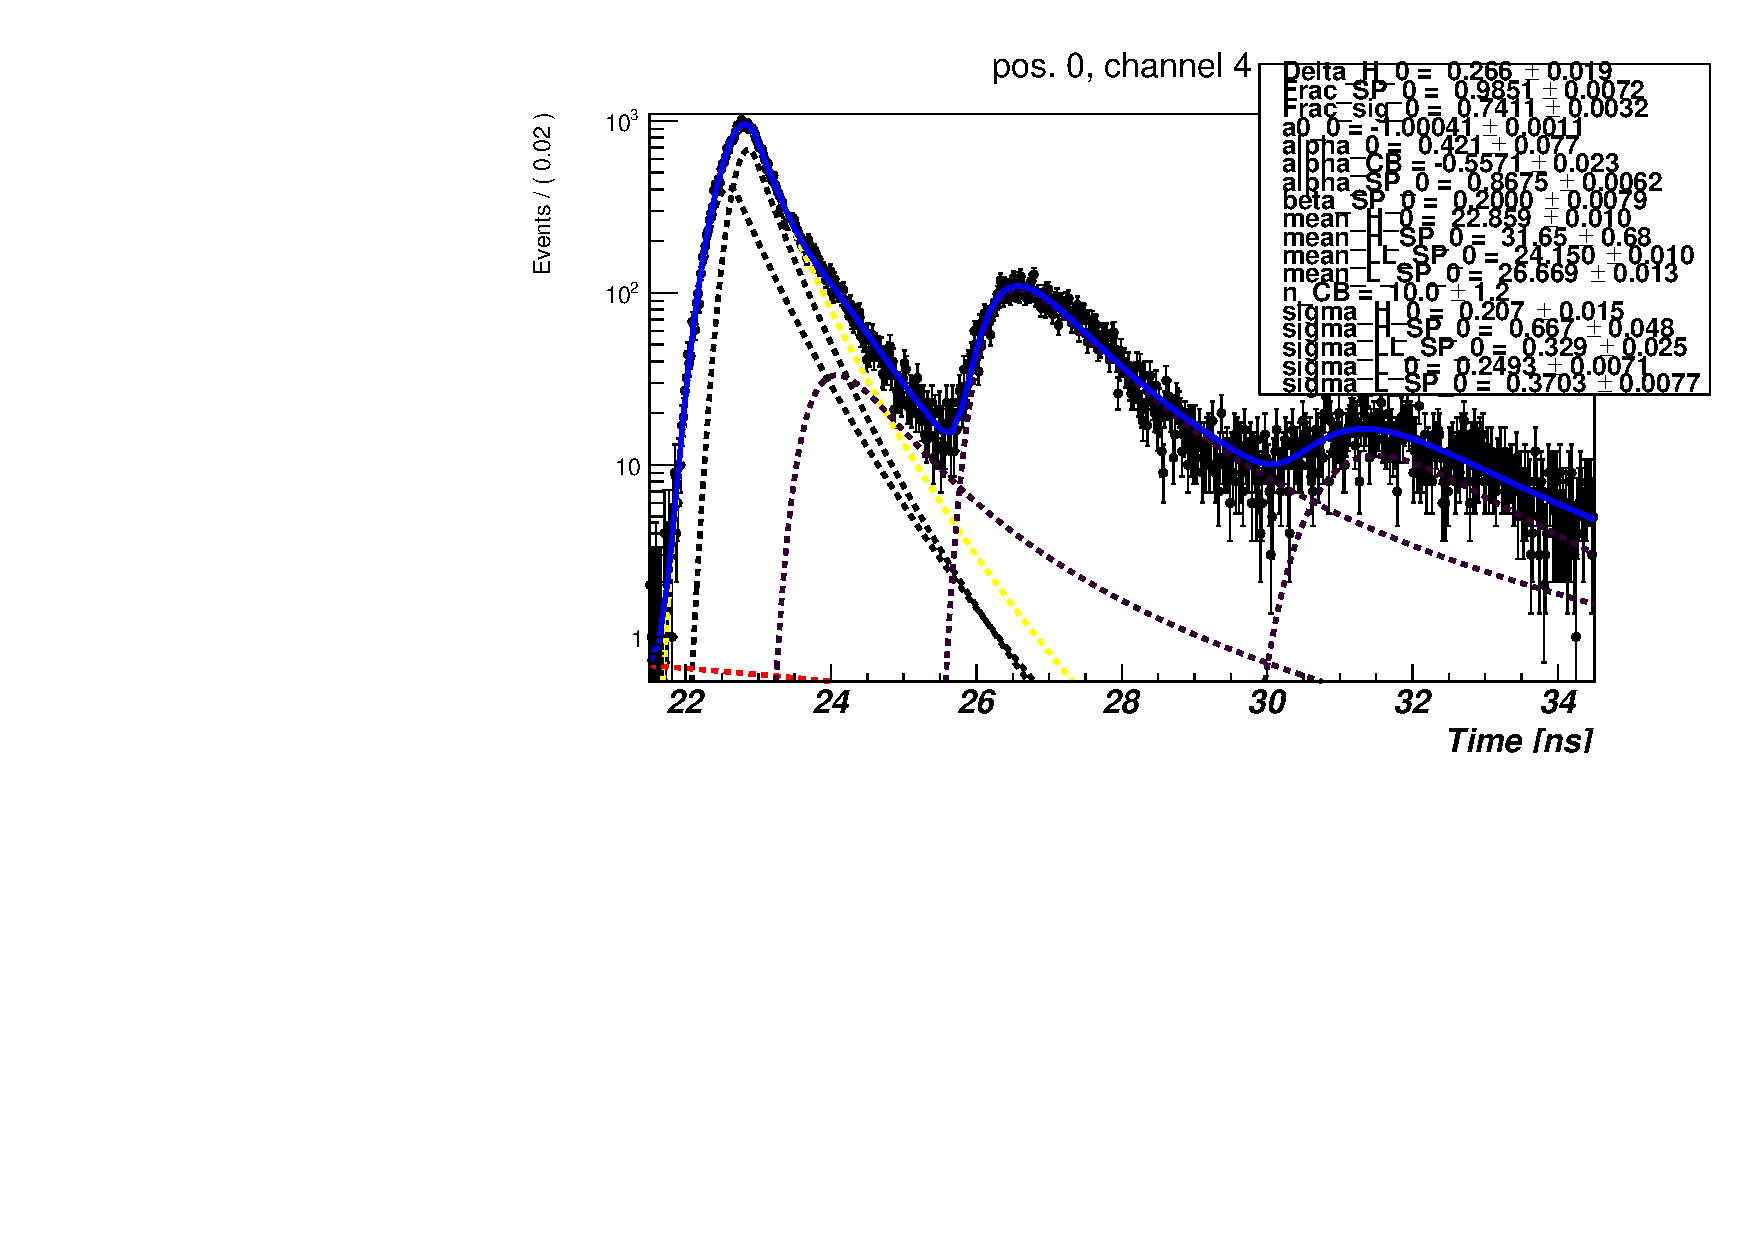
\includegraphics[scale=0.5]{plots/ch4_T86}
\caption{Time spectra observed in a MCP-PMT pixel, acquired with a laser tune value of 86\%.}
\label{fig:SP_MCPPMT_T86}
\end{center}
\end{figure}

\begin{figure}
\begin{center}
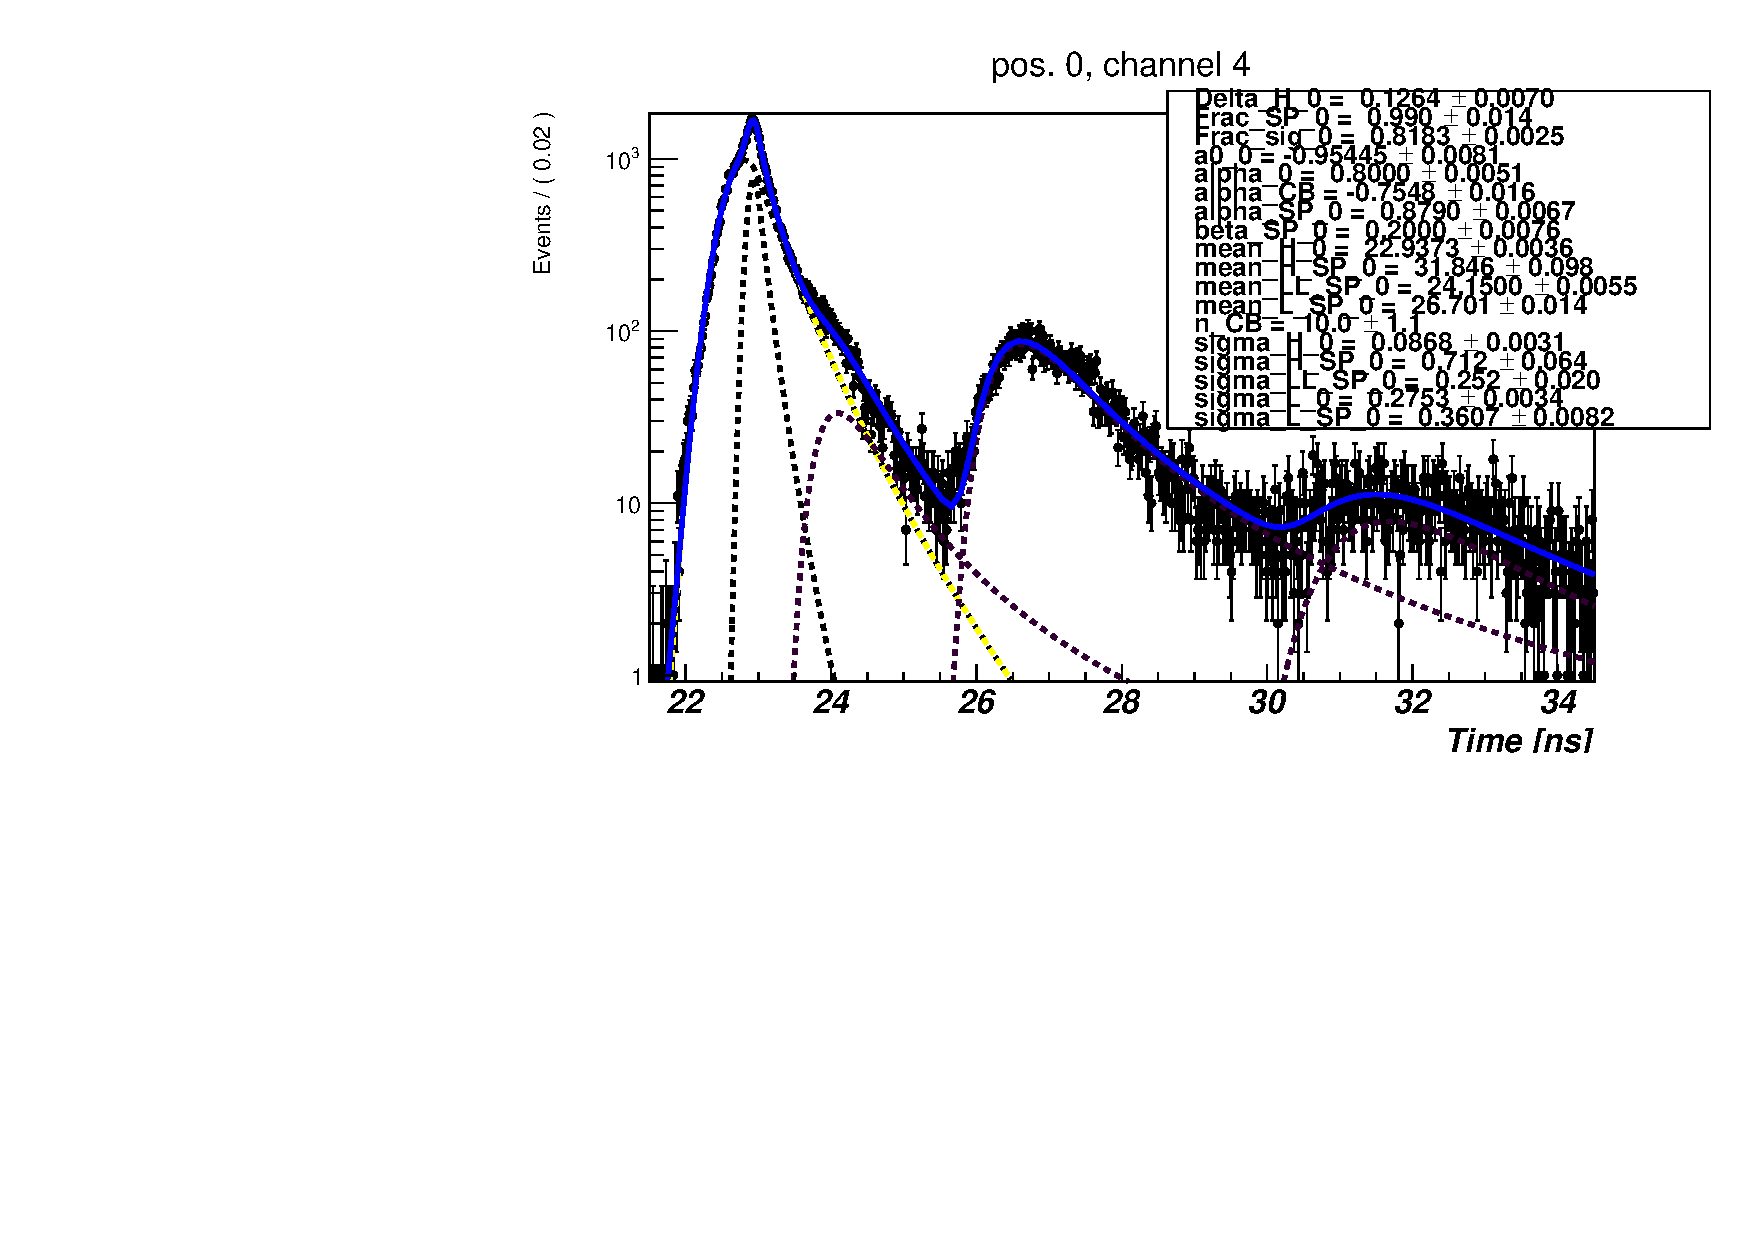
\includegraphics[scale=0.5]{plots/ch4_T80}
\caption{Time spectra observed in a MCP-PMT pixel, acquired with a laser tune value of 80\%.}
\label{fig:SP_MCPPMT_T80}
\end{center}
\end{figure}


\begin{figure}
\begin{center}
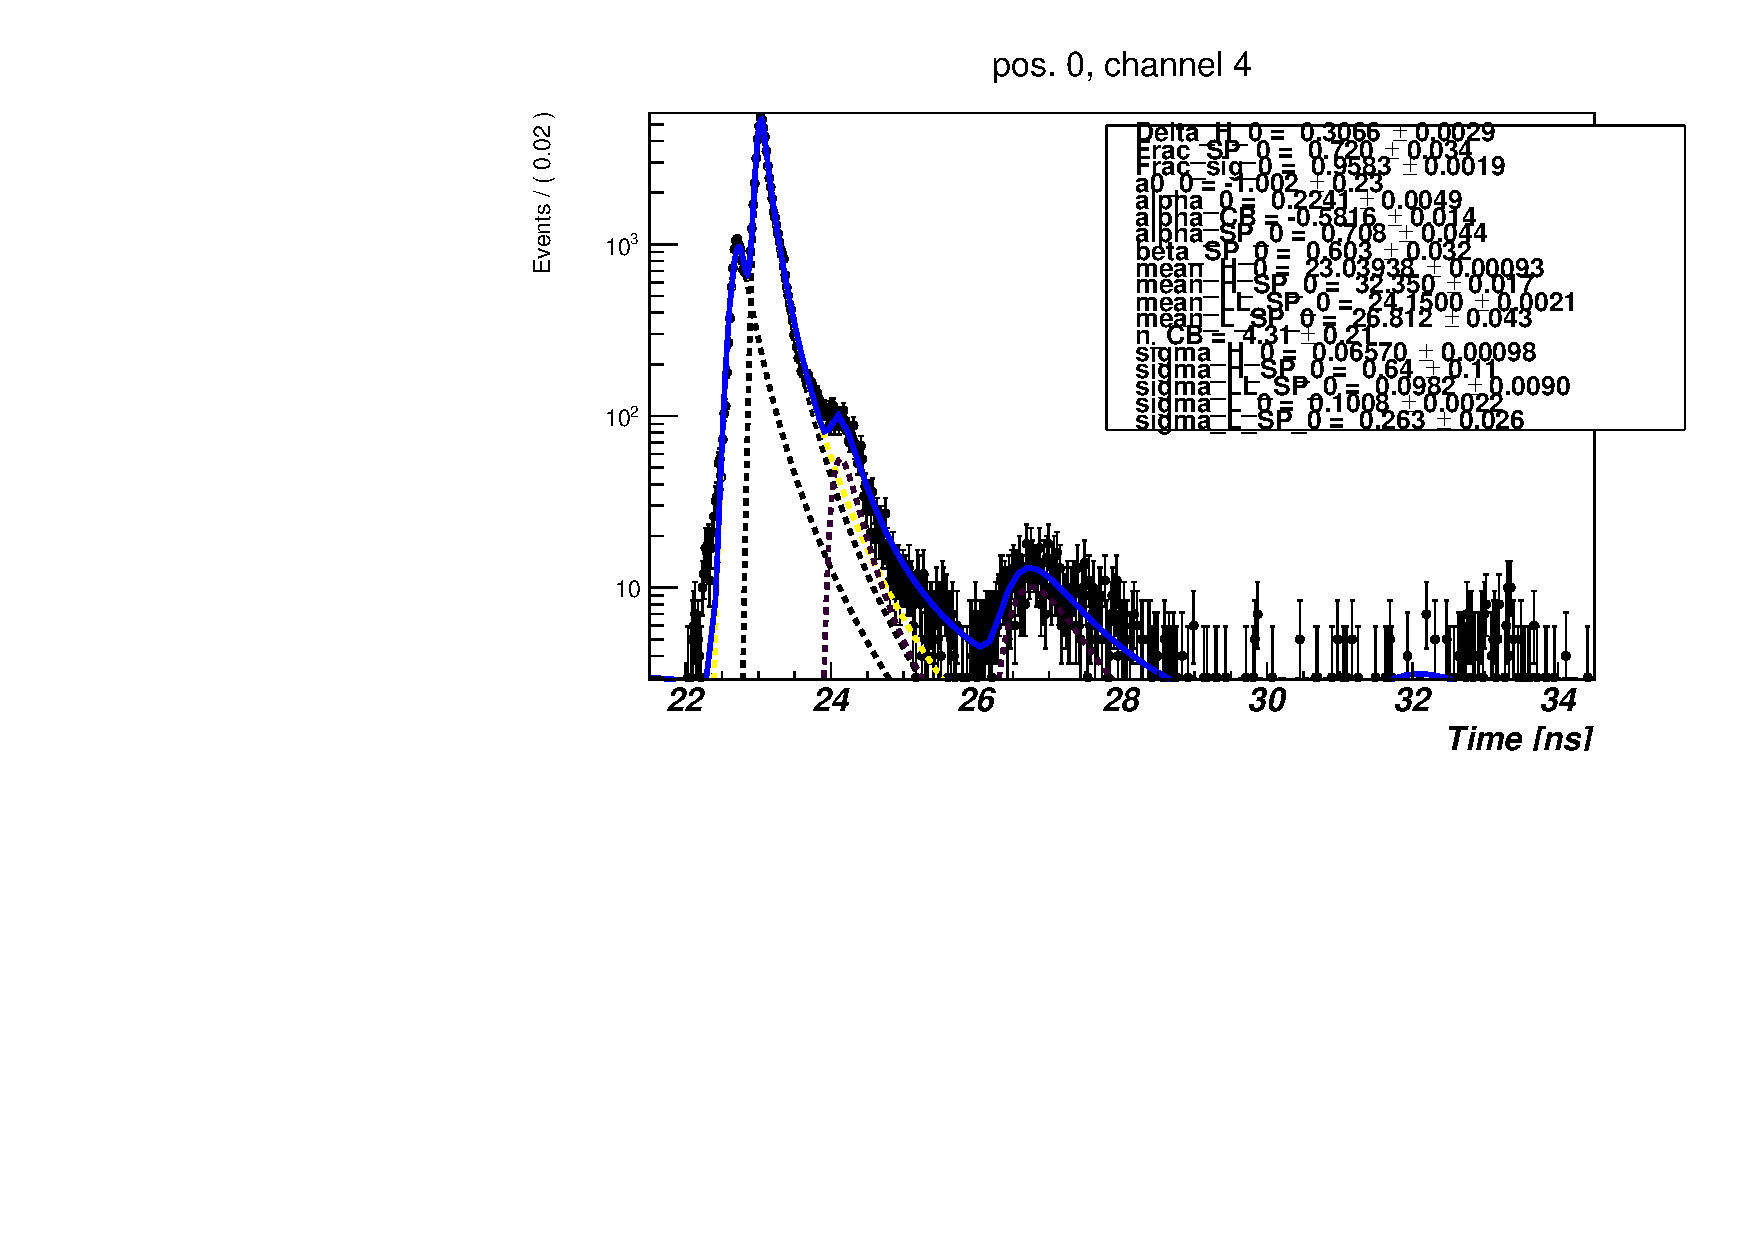
\includegraphics[scale=0.5]{plots/ch4_T77}
\caption{Time spectra observed in a MCP-PMT pixel, acquired with a laser tune value of 77\%.}
\label{fig:SP_MCPPMT_T77}
\end{center}
\end{figure}


\begin{figure}
\begin{center}
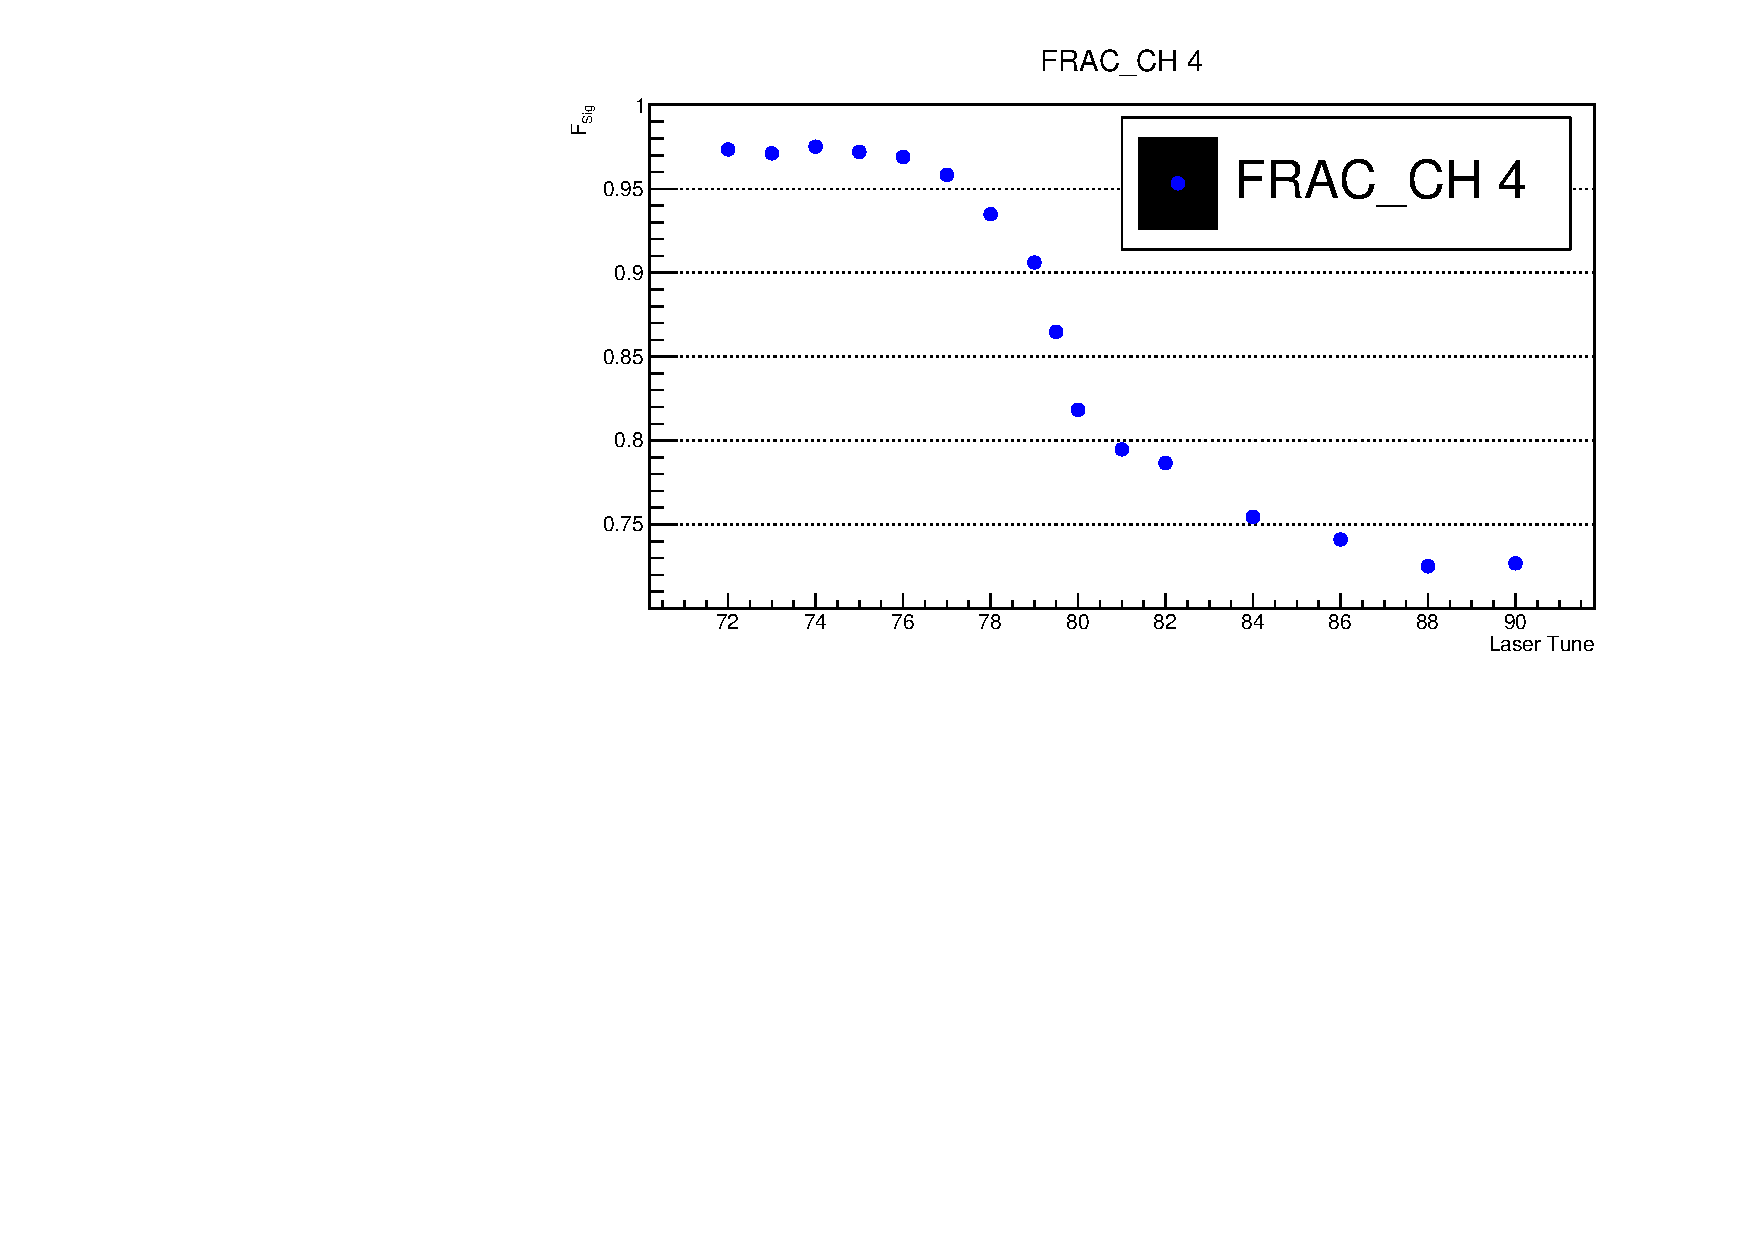
\includegraphics[scale=0.7]{plots/Fsig_ch4}
\caption{Total fraction of main emission photon signals as a function of the laser tune value, measured in one of the 16 MCP-PMT pixels. The error bars are within the point sizes. }
\label{fig:SP_MCPPMT}
\end{center}
\end{figure}
\end{subsection}

\begin{subsection}{Conclusions}
A characterization of the laser device that will be used for the iTOP calibration and monitoring has been presented.
A study of the dependence from the laser attenuation value of the photon mean emission time, time resolution, and yield of delayed emitted bunches, has been performed in order to define a suitable working point which allows to perform reliable calibration and stability monitoring. 

A high non linear dependence is observed between the above mentioned quantities and the value of the laser attenuation. Tune values smaller than $\sim 76\%$ can guarantee both a good time resolution as well as a negligible yield of delayed photon bunches. In this region, though, the single photon regime is loose and, depending on the particular needs, an external attenuation mechanism (not affecting the laser photons temporal properties) could be required.

\end{subsection}

\section{Time spectra analysis: data-driven method}

In this section the data-driven validation of the fit procedure is presented. The first action is to determine which is the shape of a single photon signal. The width of the profile function represents the time resolution that can be obtained with the employed acquisition chain. The time detection spectra of photons coming out from the expansion prism will consists of a superposition of several elementary profiles. 

In the following, in order to cut away the noise due to the delayed emitted photons, detection time spectra are analyzed in a range of $\sim$ 1 ns around the mean position of the main signal peak


\begin{subsection}{Study of single path detection time shape}

The study of the elementary signal has been performed running an acquisition with MCP-PMT placed in front of the light source, with no prism in between. The laser tune value has been set to 50\%.

Fig.\ref{fig:sig_shape_ch5} show the time detection spectrum observed in two of the 16 MCP-PMT pixels. As it is seen, the shape is highly asymmetric and non gaussian, because of a tail at high times. The functional form that fits better this shape is a {\it Crystal Ball} function, consisting of a gaussian core and a power law tail at high times. A second degree polyomial function has been added to take into account the presence of any kind of electronic or environmental noise; nonetheless, the yield of the noise component is found to be negligible. 

The measured width of the gaussian core represents the resolution in the best case scenario, namely the best can be achieved, and has values of $\sim$ 50-80 ps, depending on the acquisition chain of the pixel. The presence of the prism will have the effect of increase the time spread of the different photon paths.



%\begin{figure}
%\begin{center}
%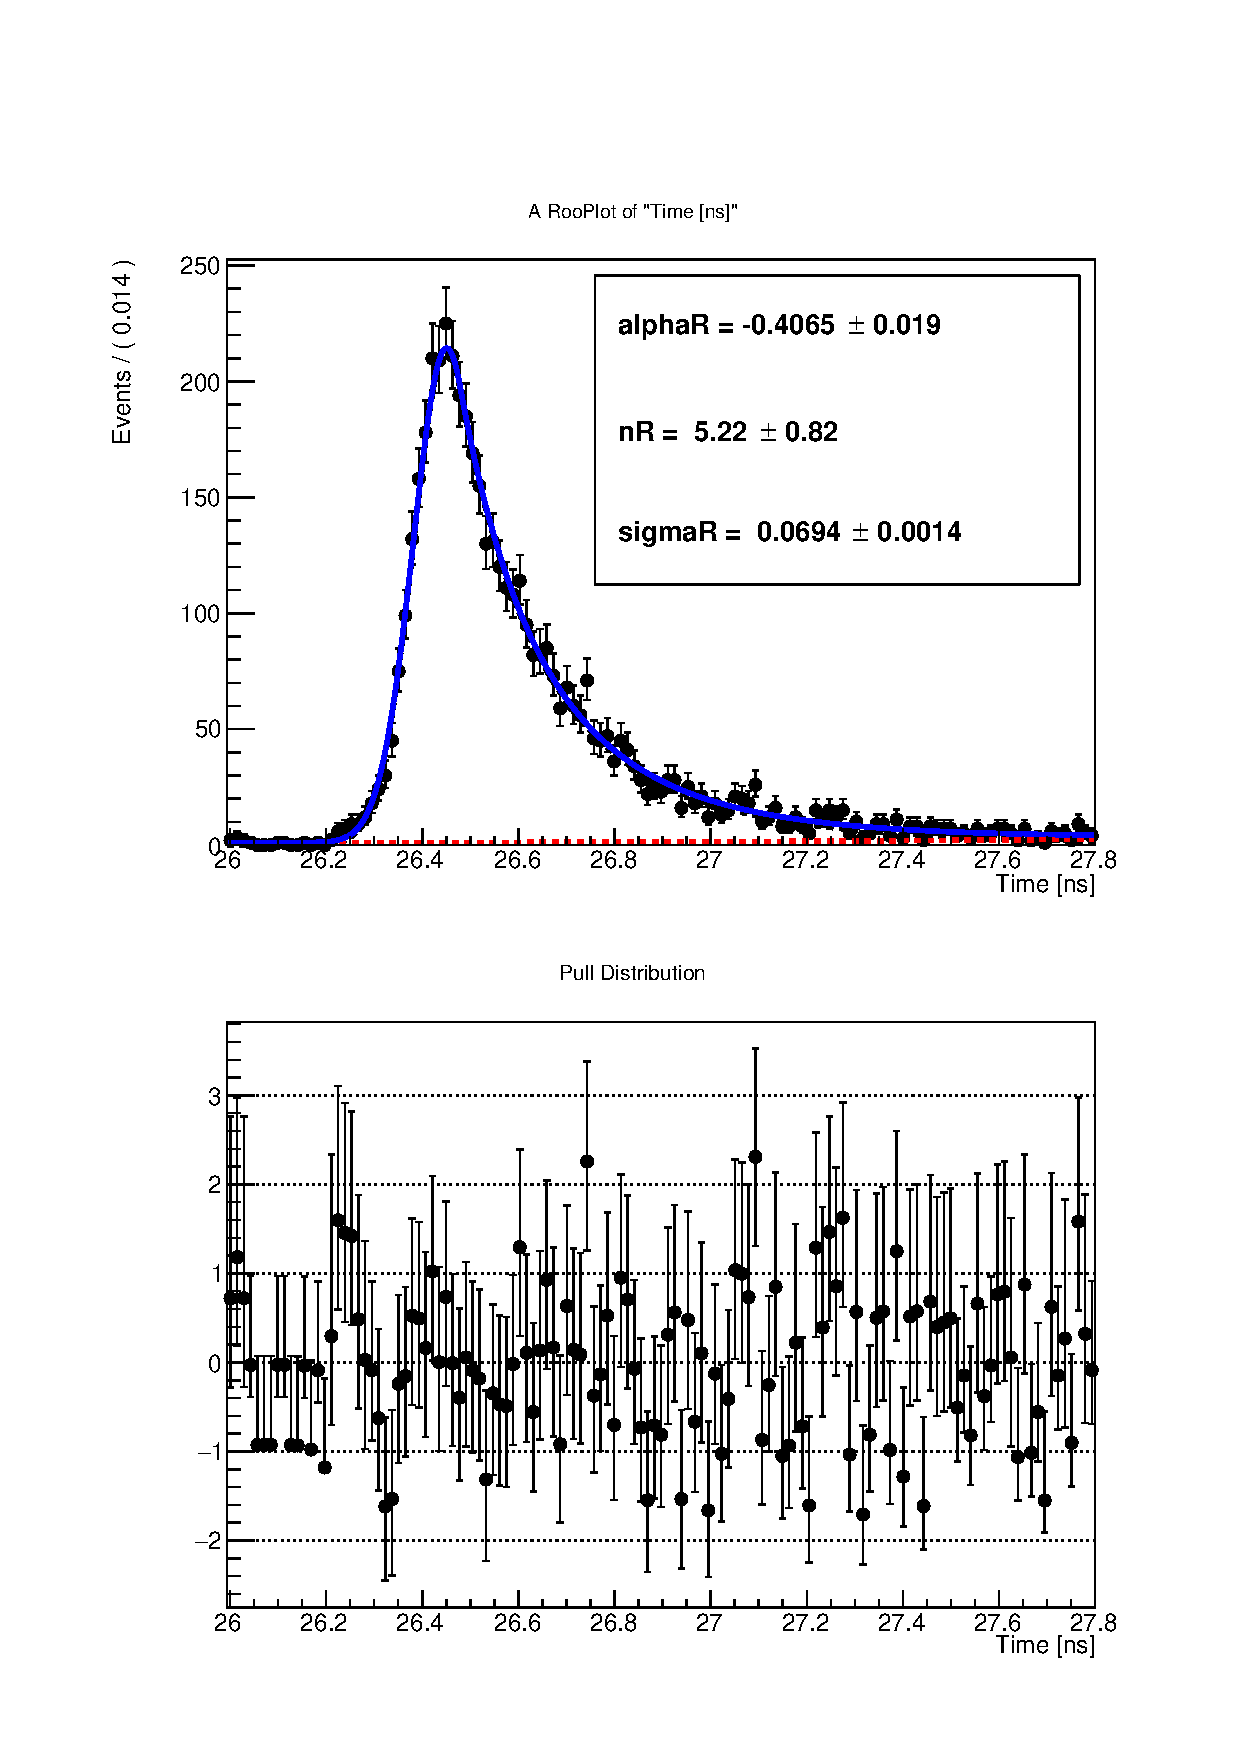
\includegraphics[scale=0.7]{plots/Sig_shape_ch2}
%\caption{Time detection spectrum }
%\label{fig:sig_shape_ch2}
%\end{center}
%\end{figure}

\begin{figure}
\begin{center}
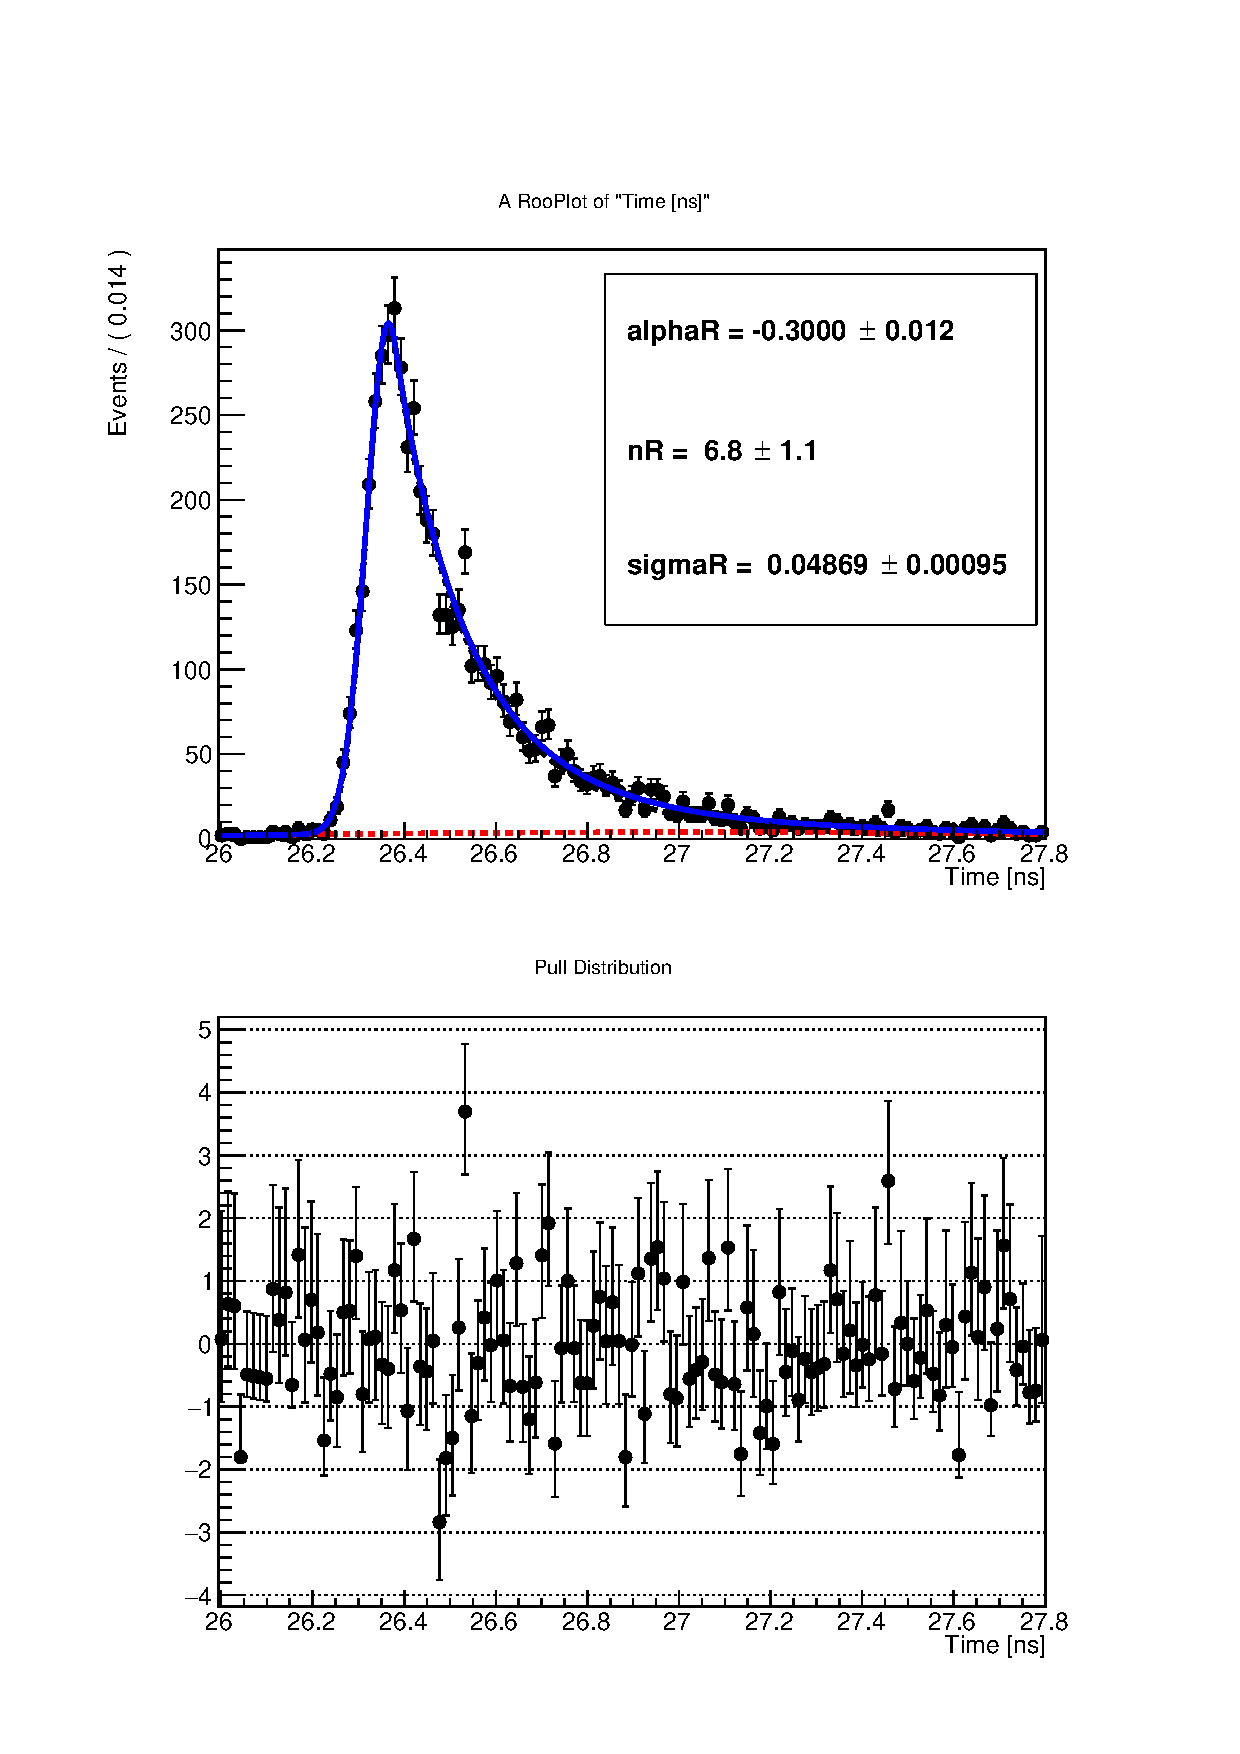
\includegraphics[scale=0.5]{plots/Sig_shape_ch5}
\caption{Time detection spectrum observed in one of the 16 MCP-PMT. The results of the fit are superimposed (signal:black dotted, noise: red-dotted, total: blue), and the fit pulls are shown in the bottom plot.}
\label{fig:sig_shape_ch5}
\end{center}
\end{figure}


\end{subsection}


\begin{subsection}{The  single fiber spectra}

As already said, the advantage of having a dedicated test bench system is that it is possible to analyze spectra from each single fiber. 

\paragraph{Data} 

\paragraph{Fit model}


\paragraph{Fit results}

\end{subsection}

\begin{subsection}{The two-fiber contribution}
\paragraph{Data}
\paragraph{Fit model}
\paragraph{Fit result}



\end{subsection}

\begin{subsection}{subsection one.1}
\begin{figure}[h]\label{fig:1d_case}
\includegraphics[scale=0.1]{D:/Padova/Presentazioni/Logos/belle2-logo.png}
\caption{\footnotesize caption}
\end{figure}
\end{subsection}


\begin{subsection}{subsection one.2}
 subsection one.2
\end{subsection}



\section{The MC modeling}
\begin{subsection}{The lens opening distribution}

\end{subsection}
\begin{subsection}{Simulation results - Padova system}

\end{subsection}
\section{Conclusions}
\end{document}









